\clearpage
\section{Trabalho Desenvolvido}
\label{ch:developed}

Esta seção apresenta o trabalho realizado até o momento para auxiliar o desenvolvimento 
no projeto de pesquisa de doutorado. 

%This section presents the work carried out so far that is assisting the
%development of this doctoral research project. \autoref{sec:module} talks about
%some available software tools for performance evaluation and presents the new
%OpenFlow module for simulations. \autoref{sec:scenario} introduces the proposed
%\ac{SDN}-enabled \ac{LTE} simulation scenario, describing its design targets
%and the network topology. Finally, \autoref{sec:controller} describes the
%enhanced OpenFlow controller for the \ac{SDN}-enabled \ac{LTE} network.
% The work presented here is potential precursor of this doctoral research
% project.


%-----------------------------------------------------------------------------%
%\subsubsection{Comparison between the developed works}
%\label{subsec:applications}
%
%In this part, we provide a feature comparison between various state-of-the-art bitrate
%adaptation schemes in each category from the taxonomy in Figure 3.1. Table 3.1 summarizes
%this comparison for each surveyed paper in terms of the following aspects:

%-----------------------------------------------------------------------------%
\subsection{Formulação de Programação Linear Inteira~(ILP)}
\label{subsec:applications}

Um formulação de programação linear inteira pode ser modelada como um caso simples de balanceamento de carga em uma rede multinível Névoa/Nuvem para streaming de video.
Suponha que existe $n$ usuários conectados na rede, $m$ servidores de streaming de videos e $c$ streaming de video, nós queremos encontrar um \textit{matching} apropriado entre eles. Um \textit{matching} entre um usuários, servidores e videos é dado por uma tripla $(i,j,k)$. Neste caso a tripla pode ser entendida como uma sessão aberta de streaming de video atraves do protocolo HTTP. O conjunto de usuários, servidores e videos são denotados por $U$, $N_{h}$, $V$, respectivamente.
Os vértices representam nós de rede e as arestas são os links de rede podendo ser com ou sem fio. Os links podem ser definidos por conexões físicas ou virtuais

\begin{itemize}
\item $\forall (i,j,k) \in S$, $i \in U$ e $j \in S_{c}$ e $k \in V$.

\item $\forall i \in U$, exite no maximo um par $(i,j) \in S$.

\item $\forall j \in S_{c}$, exite no maximo uma tripla $(i,j) \in S$.

\item $\forall j \in V$, exite no maximo uma tripla $(i,j) \in S$.
\end{itemize}

%Com $V$ sendo o conjunto de todos os vertices, definimos uma atribuição $S$ como um conjunto de triplas $(i,j,k)$, considerando a arquitetura da Figura~[1]:

%\begin{itemize}
%\item $\forall (i,j,k) \in S$, $i \in D$ and $j \in U$ e $k \in V$.
%
%\item $\forall i \in D$, exite no maximo uma tripla $(i,j,k) \in S$.
%
%\item $\forall j \in U$, exite no maximo uma tripla $(i,j,k) \in S$.
%
%\item $\forall k \in V$, exite no maximo uma tripla $(i,j,k) \in S$ $\forall i \in M_{D}(i)$.
%\end{itemize}
 
A progamaçãpo com o balancemanto de carga   
A programação com reconhecimento de QoS resolve um programa inteiro linear que busca o valor da variável $x_{i,j,k} (\in (0, 1))$. $x_{i,j}$ é uma variável binária que assume os seguintes valores,

\vspace{0.5cm}
\begin{equation}\label{total_capacity_loss}
x_{i,j} =
\left\{\begin{matrix}
1, & \text{se um video k é requisitado a um usuário \textit{i} no servidor \textit{j}} & \\ 
0, & \text{Caso contrário} & 
\end{matrix}\right.
\end{equation}
\vspace{0.5cm}

Em uma arquitetura multinível, os streamings de video tem um QoE diferente de acordo com os seus requisitos. Por exemplo, streaming em tempo real, como detecção on-line e streaming armazenado fim-a-fim, são sensíveis a atrasos. Portanto, esses streamings devem ser processados o mais próximo possível do usuário final, de preferência em nós localizados no primeiro nível da névoa, enquanto que conteudos de video sob Demanda~(VoD) aceitam um atraso maior. Desta forma, vamos identificar cada stream de video requisitado pelos usuários finais por um identificador, a partir de agora simbolizado por "c".
Um nível de servidores, indicado por $S_{c}$, é um conjunto de nós que atende o QoE necessário para fornecer serviços de um stream de video específico, e nós definimos como um intervalo na forma de $S_{c} \in [a, b)$. onde $a_{c} < b_{c}$ e,

\vspace{0.5cm}
\begin{itemize}

\item  $c \in \{1,...,v\}$

\item  $a_{c} = \{a_{1},a_{2},...,a_{v}\}$

\item  $b_{c} = \{b_{1},b_{2},...,b_{v}\}$

\item  $a_{c},b_{c} \in N_{H}$

\end{itemize}
\vspace{0.5cm}

%Para simplificar esta formulação nós estamos considerando que os segmentos de video é requisitado a apenas um servidor fonte, e utiliza um interval de tempo discreto. Assim, $T = {1, ..., T max }$, onde $T_{max}$ é o tempo maximo que o video levaria para executar no nós mais rapido da fog. $T_{max}$ pode ser calculado como 
%
%\begin{equation}\label{minimize}
%T_{max} = \sum^{m}_{k} min(TI_{k | k \in N_{H}})
%\end{equation}

%Para melhor a latência da reprodução do video, nós devemos  minimizar a latencia de um nó para todas requisiçoes de segmentos do video. 

Para simplificar esta formulação nós estamos considerando que os segmentos de video são requisitados a apenas um servidor fonte, bem como o serviço de video streaming já está em execução em seus respectivos servidores. Colocando as limitações abaixo:% An initial approach to the QoS-aware schedule is given by the following optimization problem:


\vspace{0.5cm}

%\begin{equation}\label{minimize}
%\text{minimize} \ \ \
%\sum^{\left | D \right |}_{i=1} 
%\sum_{\{j | (i,j,k) \in A\}}
%\sum_{\{k | (i,j,k) \in A\}}
%\frac{ c_{ijk} }{ m_{i}} \ast x_{ijk}
%\end{equation}

Minimizar

\begin{equation}\label{maximize}
\sum_{i \in U} 
\sum_{j \in S_{c}}
\sum_{k \in V}
a_{ij} \ast x_{ijk}
\end{equation}

Sujeito a

\begin{equation}\label{bound_1}
%\sum_{\{j | (i,j,k) \in A\}}
\sum_{ j \in S_{c} }
\sum_{ j \in V}
x_{ijk} = 1,  \forall i \in U
\end{equation}

\begin{equation}\label{bound_1}
%\sum_{\{j | (i,j,k) \in A\}}
%\sum_{\{ | (i,j,k) \in A\}}
\sum_{ j \in U}
\sum_{ k \in V }
x_{ijk} \leq 1,  \forall j \in S_{c}
\end{equation}

\begin{equation}\label{minimize}
\sum_{i \in U}
\sum_{j \in S_{c}}
bw_{j} x_{ij}
\leq Bw_{j}
\end{equation}

\begin{equation}\label{minimize}
x_{ij}  \in  \{0, 1\}, \forall i \in U,j \in S_{c}
\end{equation}

\begin{equation}\label{minimize}
Bw_{j} \geq  0, \forall j \in S_{c}
\end{equation}
\vspace{1.2cm}

Para melhorar o desempenho da rede assossiamos uma latencia $a_{ij}$, desta forma, nós devemos atribuir todos os usuários aos respectivos streaming de video afim de minimizar a latencia total.
%A função objetivo minimiza o makepan do aplicativo fornecido por um planejamento.
%Para melhorar a latência da reprodução do video, nós devemos  minimizar a latencia de um nó para todas requisiçoes de segmentos do video. 
Logo, a função objetivo busca essa minimização. A primeira restrição requer que cada usuário seja atribuído a exatamente um servidor. A segunda restrição garante que cada usuário seja atribuído a no maximo um servidor. Afirma também que, se o número de sessões abertas dentro de um servidor é maior do que o número de usuários atendidos, alguns dos videos permanecem sem atribuição. A terceira restrição garante que os slots de download em uma similaridade com a classe de download diferem de segmentos de video requisitados.

A Restrição (5) estabelece as restrições de capacidade de comprimento de banda que evita a atribuição de mais streaming de video do que a capacidade total disponível para cada nó de névoa.

A restrição (6) define o domínio para a variável $x_{j, t, k}$ na formulação. A restrição (6) estabelece que s variável $Bw$ deve ser números inteiros não negativos.

%-----------------------------------------------------------------------------%
\subsection{Avalização sobre o provisionamento de Video em Diferentes Níveis}
\label{subsec:evaluation}

Algumas simulações foram realizadas para investigar como o as diferenças no algorimos implantados em serviços DASH no lado do cliente se comportam:~\textit{i)} Rate: O controlador ABR solicita a taxa de bits mais alta
que a rede pode suportar com base na estimativa de largura de banda disponível obtida de segmentos baixados anteriormente;~\textit{ii)} Buffer: O controlador ABR usa a ocupação do buffer de reprodução para selecionar uma taxa de bits adequada para futuros pedaços que mantêm o buffer no nível de ocupação desejado;~\textit{iii)} Hybrid: Esse tipo de controlador ABR combina as duas heurísticas mencionadas acima para decidir qual o nível de taxa de bits do próximo bloco a ser baixado.
 

%mecanismos de controle podem trabalhar juntos na rede LTE habilitada para SDN.

Para implementar os servidores DASH e os usuários que permitem o streaming de video adaptativo, modificamos o  Adaptive Multimedia Streaming com a base de código AMuSt~(AMuSt). 
A estrutura do AMuSt fornece um conjunto de aplicativos para produzir e consumir vídeo adaptável, com base no padrão DASH~\cite{kreuzberger2016amust}. A funcionalidade do DASH é fornecida pela biblioteca libdash~\cite{mueller2013ICMEW}, uma biblioteca de código aberto que fornece uma interface para o padrão DASH. Atualmente, libdash é o software de referência oficial do padrão DASH.
Considemoramos que os usuários estão interessado em um vídeo disponível com dez representações diferentes, de taxa de bits \{235kbps, 375kbps, 560kbps, 560kbps, 750kbps, 1050kbps, 1750kbps, 2350kbps, 3000kbps, 4300kbps, 5800kbps\}, que são um subconjunto dos usados pela Netflix no passado~\cite{netflix:representation}.
Cada representação é dividida em segmentos de 2 segundos. Cada experimento foi executado 10 vezes com tempo do execução de 600 segundos.

%We consider that the end-users are interested in a video available in three different representations, Q = \{480p, 720p, 1080p\} with bitrates \{1750kbps, 3000kbps, 5800kbps\}, respectively, that are a subset of the ones used by Netflix in the past [11]. Each representation is divided into a set of 50 segments, each of a duration of 2 seconds.

%Primeiro, focamos em um cenário de rede de caminhos múltiplos simples (consulte
%Fig. 2), onde os usuários estão conectados a quatro repositórios por quatro caminhos não disjuntos. Usuários no nó de acesso exclusivo 

%\vspace{0.8cm}
\begin{figure*}[htpb]
	\centering
	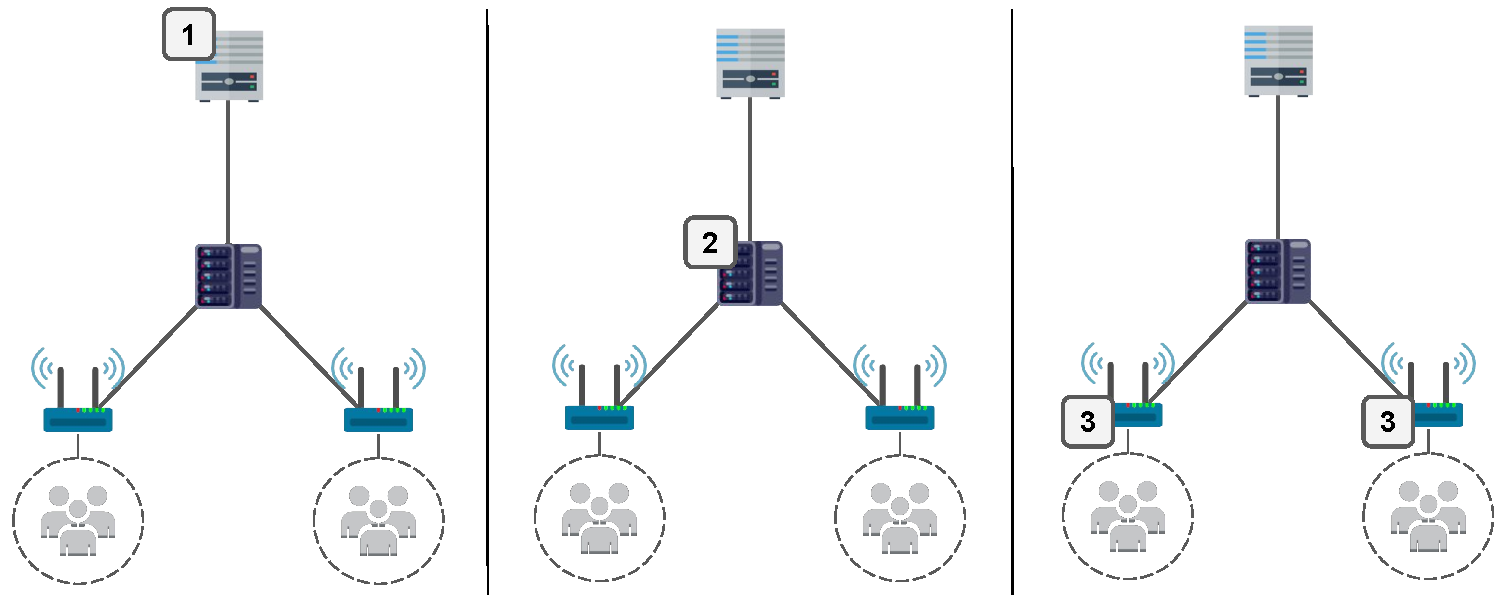
\includegraphics[width=0.75\textwidth]{img/exp-multi-lvl}
% 	\vspace{-1cm}
	\caption{DASH-based Adaptive Multimedia Delivery System for Cloud/Fog Nodes.}
	\label{fig:scenario-arch}
\end{figure*}
%\vspace{0.8cm}

As Figuras 4(a) e 5(a) mostram a taxa de bits media~(Bandwidth Blocking Ratio) com 20 e 40 usuários, respectivamente. No cenario com 20 usuários~(Figura 4(a)) as tres heuristicas ABR apresentam um impacto semelhante. Enquanto que, intuitivamente, o provisionamente do video DASH entre os níveis 1 e 2 apresentam uma diferença estritamente superior, em contrapartida, o nível 3 apresenta uma disparaidade significativa em relação aos outros niveis. Para o cenario com 40 usuarios a taxa de bits medio entre niveis apresentam uma diferenças semelhantes em ordem de grandeza. 

As Figuras 4(b) e 5(b) mostram o tempo de interrupção total~(Bandwidth Blocking Ratio) com 20 e 40 usuários, respectivamente. Ao contrario da taxa de bit media, aqui nós podemos observar uma diferença em relação aos mecanismos ABR no cenario com 20 usuários~(Figura 4(a)), principalmente, quando o video é provisionado por um servidor no nivel com mais saltos~(nível 1). Este comportamento é suvisado no cenario com 40 usuarios, onde existe uma pequena diferenca ente os mecanismos de decisao no nivel 2.


É importante notar que apesar do bitrate medio entre os mecanismos ABR serem semelhantes, as interrupções que eles podem gerar são significativamente diferentes, o que impacta diretamente no QoE dos usuários. Outro ponto a ser observado é a taxa de bits media entre os diferentes niveis. No cenario com 20 usuários o nivel 3 conseguiu atingir o que necessario para obter a representação de maior taxa bits.

%entre os 
% diferença de npirveis há o mesmo pode ser observado no segundo cenario co 40 usuários. Uma diferença interessante 
%
%
%Avaliamos o impacto que uma arquitetura multinível de streaming de vídeo adaptativo em uma topologia com tres níveis com um único caminho, apresentada na Fig. 5. Os links possuem comprimento de possui um taxa de dados de 10 MBps e cada AP .


%\vspace{0.8cm}
\begin{figure}[htb]
  \centering
    \subfloat[Taxa de bits medio.]
    {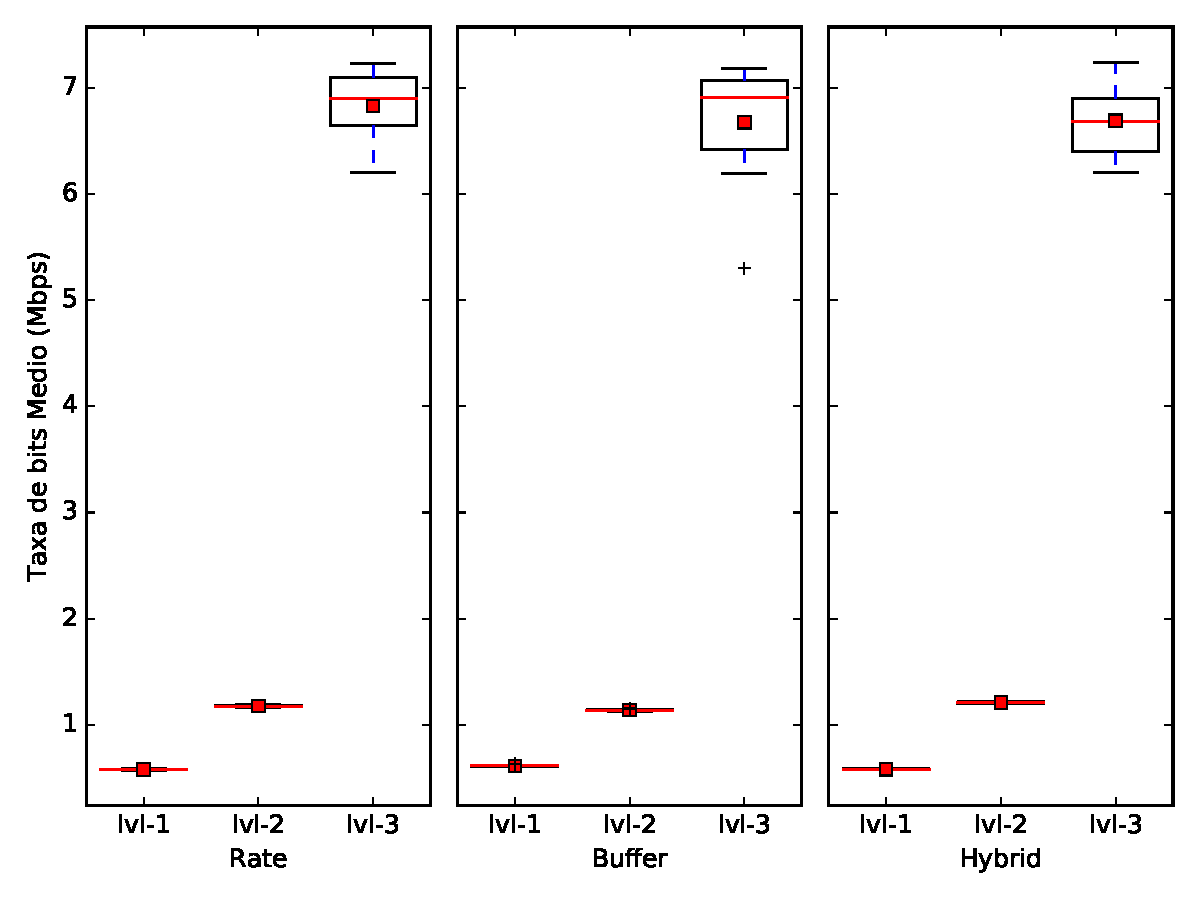
\includegraphics[width=.45\textwidth]{graphs/boxplot-avgBt-10u}
    \label{fig:lte-handover}}
  \hfil \hspace{1cm}
    \subfloat[Tempo total de interrupções.]
    {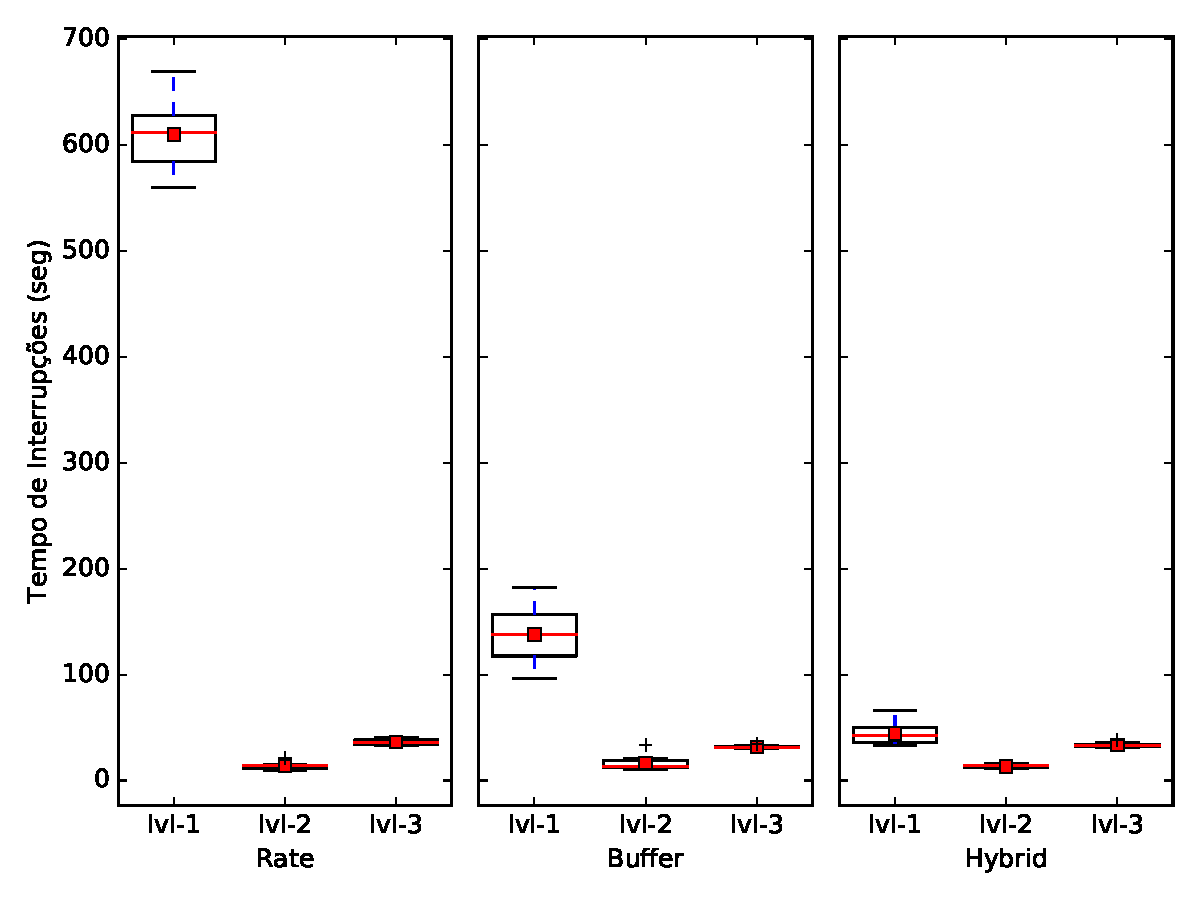
\includegraphics[width=.45\textwidth]{graphs/boxplot-avgStalls-10u}
    \label{fig:dmm-proposal}}
  \caption{Resultados da taxa de bits media e tempo total de interrupções para uma rede com 10 em cada AP.}
  \label{fig:dmm}
\end{figure}

\begin{figure}[htb]
  \centering
    \subfloat[Taxa de bits medio.]
    {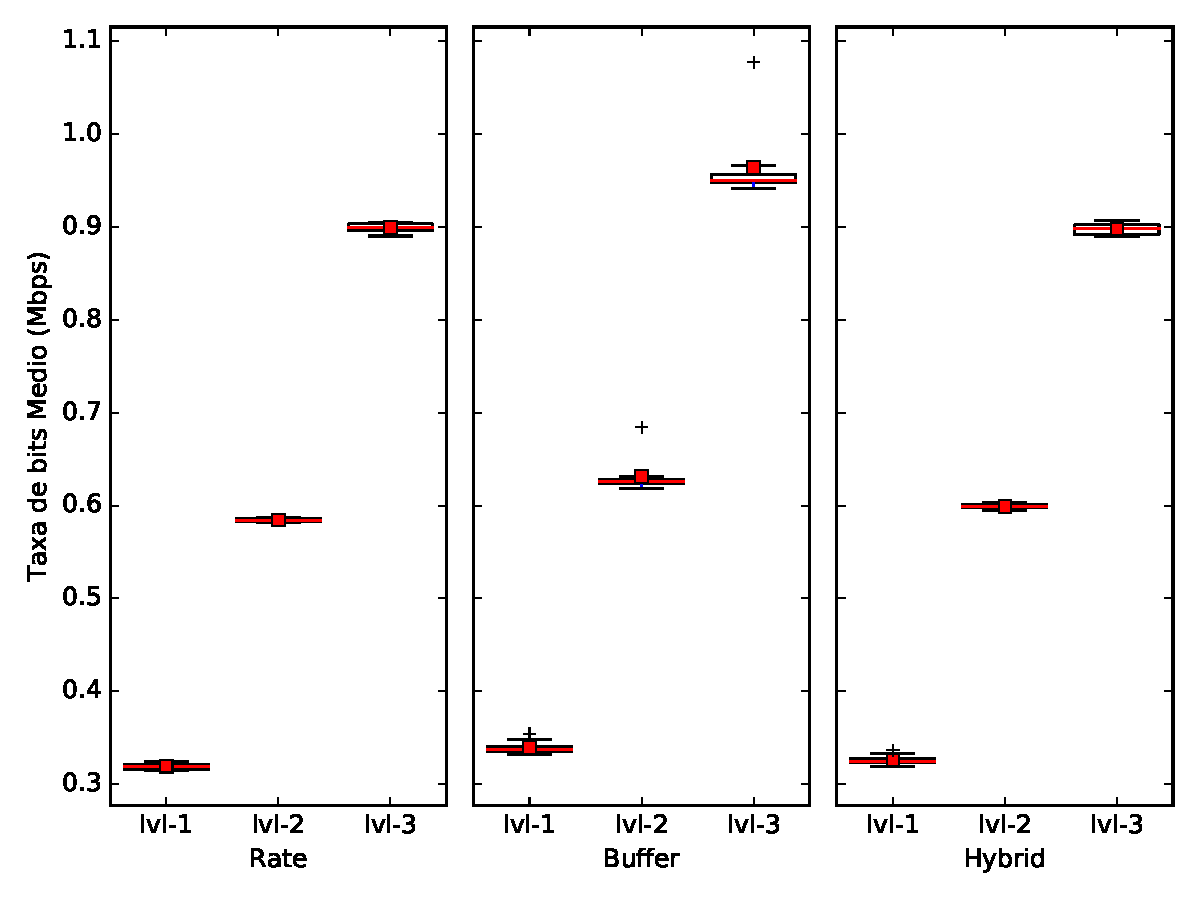
\includegraphics[width=.45\textwidth]{graphs/boxplot-avgBt-20u}
    \label{fig:lte-handover}}
  \hfil \hspace{1cm}
    \subfloat[Tempo total de interrupções.]
    {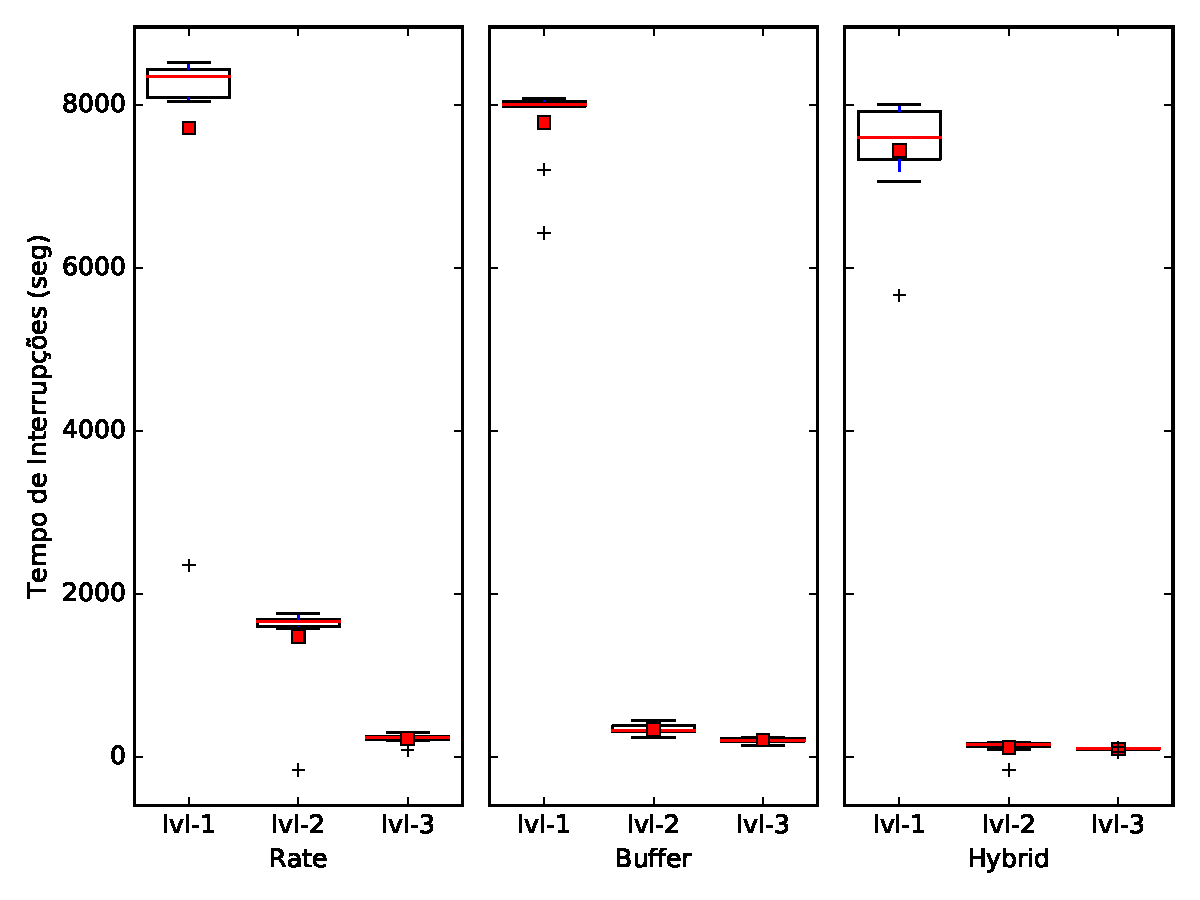
\includegraphics[width=.45\textwidth]{graphs/boxplot-avgStalls-20u}
    \label{fig:dmm-proposal}}
  \caption{Resultados da taxa de bits media e tempo total de interrupções para uma rede com 10 em cada AP.}
  \label{fig:dmm}
\end{figure}